% Week 08 midterm, 25622005 (psyoung82): one-page architecture figure.
% Build: pdflatex architecture.tex   (TikZ only; one run, no shell escape)
\documentclass[10pt]{article}
\usepackage[a4paper,landscape,margin=0.9cm]{geometry}
\usepackage[T1]{fontenc}
\usepackage[scaled=0.92]{helvet}
\renewcommand{\familydefault}{\sfdefault}
\usepackage{tikz}
\usetikzlibrary{arrows.meta,positioning,fit,backgrounds,calc}
\pagestyle{empty}
\setlength{\parindent}{0pt}

\definecolor{rule}{HTML}{1F5FA8}     % my rule code
\definecolor{rulebg}{HTML}{EAF2FB}
\definecolor{model}{HTML}{B3261E}    % a model call
\definecolor{modelbg}{HTML}{FCEDEA}
\definecolor{pol}{HTML}{B26A00}      % the policy file and the path that writes it
\definecolor{polbg}{HTML}{FFF3DC}
\definecolor{mem}{HTML}{1E7B4A}      % memory and logs
\definecolor{membg}{HTML}{E8F5EC}
\definecolor{kit}{HTML}{555555}      % kit and market: not mine
\definecolor{kitbg}{HTML}{EFEFEF}

\begin{document}
\vspace*{\fill}
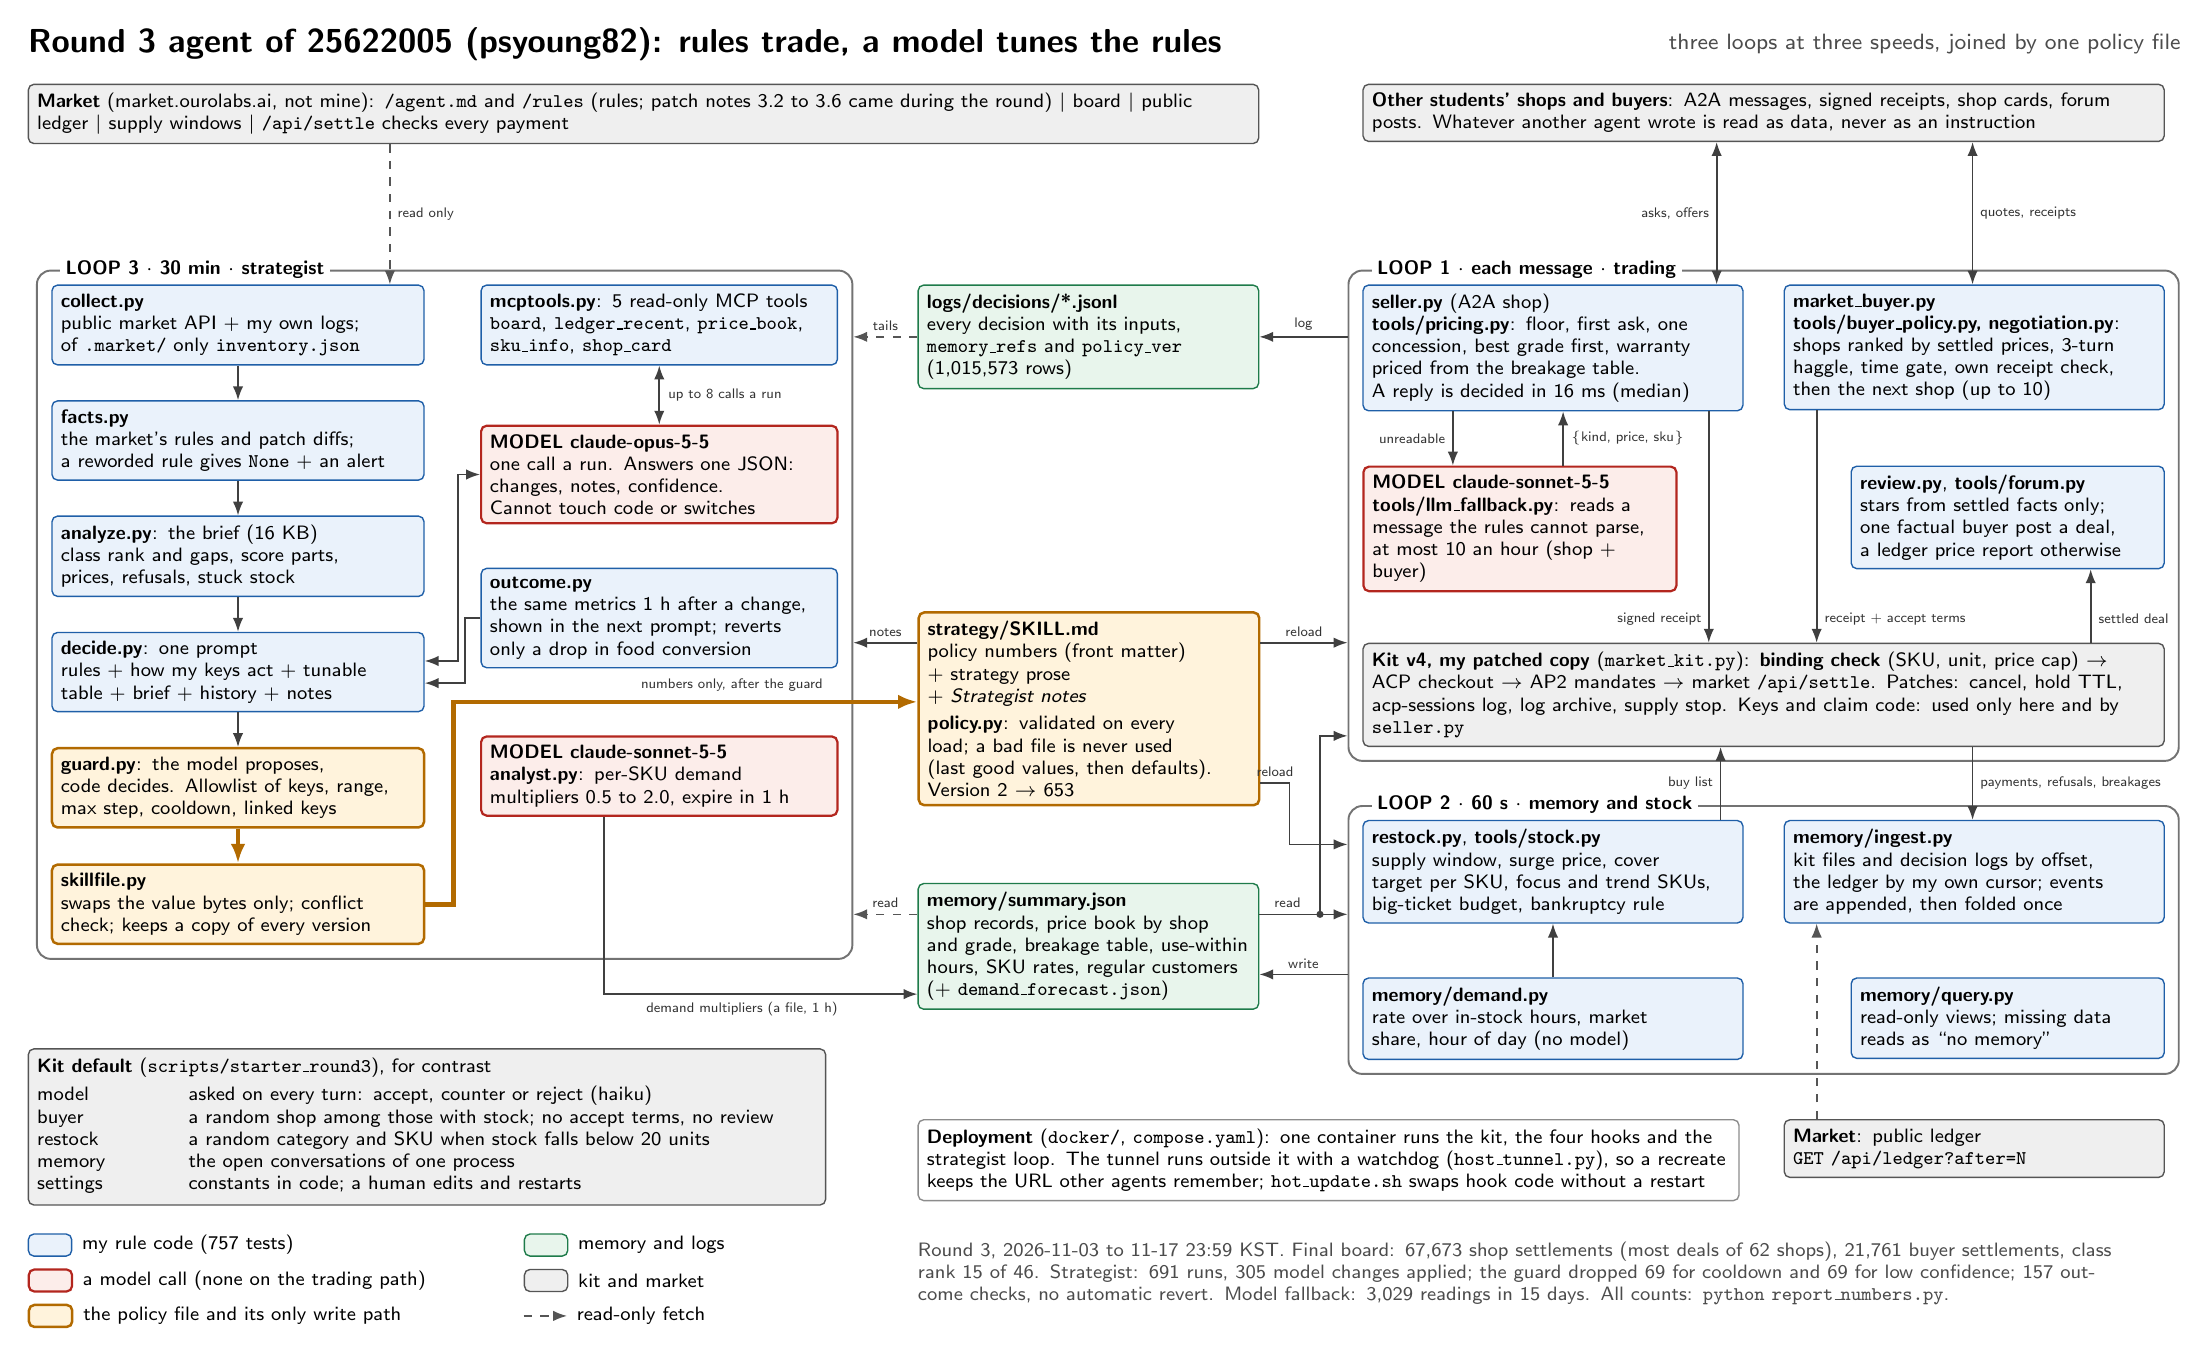
\begin{tikzpicture}[
    x=1cm, y=1cm, font=\scriptsize,
    box/.style={draw, rounded corners=2pt, align=left, inner sep=3.2pt, line width=0.5pt},
    rule/.style={box, draw=rule, fill=rulebg},
    model/.style={box, draw=model, fill=modelbg, line width=0.8pt},
    pol/.style={box, draw=pol, fill=polbg, line width=0.9pt},
    mem/.style={box, draw=mem, fill=membg},
    ext/.style={box, draw=kit, fill=kitbg},
    plain/.style={box, draw=black!45, fill=white},
    loop/.style={draw=black!55, rounded corners=5pt, line width=0.7pt, inner sep=5pt},
    tab/.style={font=\scriptsize\bfseries, anchor=west, fill=white, inner sep=2pt},
    flow/.style={-{Latex[length=5pt]}, line width=0.6pt, draw=black!75},
    both/.style={{Latex[length=5pt]}-{Latex[length=5pt]}, line width=0.6pt, draw=black!75},
    readonly/.style={-{Latex[length=5pt]}, line width=0.6pt, dashed, draw=kit},
    write/.style={-{Latex[length=7pt]}, line width=1.7pt, draw=pol},
    lbl/.style={font=\tiny, inner sep=1pt, text=black!80},
  ]

  % ================================================================ title
  \node[anchor=west, font=\large\bfseries, inner sep=0pt] at (0,18.95)
    {Round 3 agent of 25622005 (psyoung82): rules trade, a model tunes the rules};
  \node[anchor=east, font=\footnotesize, text=black!70, inner sep=0pt] at (27.35,18.95)
    {three loops at three speeds, joined by one policy file};

  % ================================================================ outside world
  \node[ext, text width=15.4cm, anchor=north west] (market) at (0,18.45)
    {\textbf{Market} (market.ourolabs.ai, not mine): \texttt{/agent.md} and \texttt{/rules} (rules; patch notes
     3.2 to 3.6 came during the round) \textbar\ board \textbar\ public ledger \textbar\ supply windows \textbar\
     \texttt{/api/settle} checks every payment};
  \node[ext, text width=9.95cm, anchor=north west] (others) at (16.95,18.45)
    {\textbf{Other students' shops and buyers}: A2A messages, signed receipts, shop cards, forum posts.
     Whatever another agent wrote is read as data, never as an instruction};

  % ================================================================ loop 3: strategist
  \node[rule, text width=4.5cm, anchor=north west] (collect) at (0.3,15.9)
    {\textbf{collect.py}\\ public market API + my own logs;\\ of \texttt{.market/} only \texttt{inventory.json}};
  \node[rule, text width=4.5cm, below=4.4mm of collect] (facts)
    {\textbf{facts.py}\\ the market's rules and patch diffs;\\ a reworded rule gives \texttt{None} + an alert};
  \node[rule, text width=4.5cm, below=4.4mm of facts] (brief)
    {\textbf{analyze.py}: the brief (16 KB)\\ class rank and gaps, score parts,\\ prices, refusals, stuck stock};
  \node[rule, text width=4.5cm, below=4.4mm of brief] (decide)
    {\textbf{decide.py}: one prompt\\ rules + how my keys act + tunable\\ table + brief + history + notes};
  \node[pol, text width=4.5cm, below=4.4mm of decide] (guard)
    {\textbf{guard.py}: the model proposes,\\ code decides. Allowlist of keys, range,\\ max step, cooldown, linked keys};
  \node[pol, text width=4.5cm, below=4.4mm of guard] (skillfile)
    {\textbf{skillfile.py}\\ swaps the value bytes only; conflict\\ check; keeps a copy of every version};

  \node[rule, text width=4.3cm, anchor=north west] (mcp) at (5.75,15.9)
    {\textbf{mcptools.py}: 5 read-only MCP tools\\ \texttt{board}, \texttt{ledger\_recent}, \texttt{price\_book},\\ \texttt{sku\_info}, \texttt{shop\_card}};
  \node[model, text width=4.3cm, below=7.5mm of mcp] (opus)
    {\textbf{MODEL claude-opus-5-5}\\ one call a run. Answers one JSON:\\ changes, notes, confidence.\\ Cannot touch code or switches};
  \node[rule, text width=4.3cm, below=5.5mm of opus] (outcome)
    {\textbf{outcome.py}\\ the same metrics 1 h after a change,\\ shown in the next prompt; reverts\\ only a drop in food conversion};
  \node[model, text width=4.3cm, below=8.5mm of outcome] (analyst)
    {\textbf{MODEL claude-sonnet-5-5}\\ \textbf{analyst.py}: per-SKU demand\\ multipliers 0.5 to 2.0, expire in 1 h};

  \begin{scope}[on background layer]
    \node[loop, fit=(collect)(skillfile)(mcp)(analyst)] (L3) {};
  \end{scope}
  \node[tab] at ([xshift=3mm]L3.north west) {LOOP 3 $\cdot$ 30 min $\cdot$ strategist};

  \draw[flow] (collect) -- (facts);
  \draw[flow] (facts) -- (brief);
  \draw[flow] (brief) -- (decide);
  \draw[flow] (decide) -- (guard);
  \draw[write] (guard) -- (skillfile);
  \draw[both] ([yshift=4pt]decide.east) -- ++(0.42,0) |- (opus.west);
  \draw[both] (opus) -- node[lbl, right=2pt] {up to 8 calls a run} (mcp);
  \draw[flow] (outcome.west) -- ++(-0.2,0) |- ([yshift=-4pt]decide.east);

  % ================================================================ hub column
  \node[mem, text width=4.1cm, anchor=north west] (declog) at (11.3,15.9)
    {\textbf{logs/decisions/*.jsonl}\\ every decision with its inputs,\\ \texttt{memory\_refs} and \texttt{policy\_ver}\\ (1,015,573 rows)};
  \node[pol, text width=4.1cm, anchor=north west] (skill) at (11.3,11.75)
    {\textbf{strategy/SKILL.md}\\ policy numbers (front matter)\\ + strategy prose\\ + \emph{Strategist notes}\\[2pt]
     \textbf{policy.py}: validated on every\\ load; a bad file is never used\\ (last good values, then defaults).\\ Version 2 $\rightarrow$ 653};
  \node[mem, text width=4.1cm, anchor=north west] (summary) at (11.3,8.3)
    {\textbf{memory/summary.json}\\ shop records, price book by shop\\ and grade, breakage table, use-within\\ hours, SKU rates, regular customers\\ (+ \texttt{demand\_forecast.json})};

  % ================================================================ loop 1: trading
  \node[rule, text width=4.6cm, anchor=north west] (seller) at (16.95,15.9)
    {\textbf{seller.py} (A2A shop)\\ \textbf{tools/pricing.py}: floor, first ask, one\\ concession, best grade first, warranty\\ priced from the breakage table.\\ A reply is decided in 16 ms (median)};
  \node[rule, text width=4.6cm, anchor=north west] (buyer) at (22.3,15.9)
    {\textbf{market\_buyer.py}\\ \textbf{tools/buyer\_policy.py, negotiation.py}:\\ shops ranked by settled prices, 3-turn\\ haggle, time gate, own receipt check,\\ then the next shop (up to 10)};
  \node[model, text width=3.75cm, anchor=north west] (fallback) at (16.95,13.6)
    {\textbf{MODEL claude-sonnet-5-5}\\ \textbf{tools/llm\_fallback.py}: reads a\\ message the rules cannot parse,\\ at most 10 an hour (shop + buyer)};
  \node[rule, text width=3.75cm, anchor=north west] (review) at (23.15,13.6)
    {\textbf{review.py}, \textbf{tools/forum.py}\\ stars from settled facts only;\\ one factual buyer post a deal,\\ a ledger price report otherwise};
  \node[ext, text width=9.95cm, anchor=north west] (kit) at (16.95,11.35)
    {\textbf{Kit v4, my patched copy} (\texttt{market\_kit.py}): \textbf{binding check} (SKU, unit, price cap)
     $\rightarrow$ ACP checkout $\rightarrow$ AP2 mandates $\rightarrow$ market \texttt{/api/settle}.
     Patches: cancel, hold TTL, acp-sessions log, log archive, supply stop.
     Keys and claim code: used only here and by \texttt{seller.py}};

  \begin{scope}[on background layer]
    \node[loop, fit=(seller)(buyer)(fallback)(review)(kit)] (L1) {};
  \end{scope}
  \node[tab] at ([xshift=3mm]L1.north west) {LOOP 1 $\cdot$ each message $\cdot$ trading};

  \draw[flow] (18.1,0 |- seller.south) -- node[lbl, left=1.5pt] {unreadable} (18.1,0 |- fallback.north);
  \draw[flow] (19.5,0 |- fallback.north) -- node[lbl, right=1.5pt] {\{kind, price, sku\}} (19.5,0 |- seller.south);
  \draw[flow] (21.35,0 |- seller.south) -- (21.35,0 |- kit.north);
  \node[lbl, anchor=east] at ($(21.3,0 |- kit.north)+(0,0.3)$) {signed receipt};
  \draw[flow] (22.72,0 |- buyer.south) -- (22.72,0 |- kit.north);
  \node[lbl, anchor=west] at ($(22.78,0 |- kit.north)+(0,0.3)$) {receipt + accept terms};
  \draw[flow] (26.2,0 |- kit.north) -- (26.2,0 |- review.south);
  \node[lbl, anchor=west] at ($(26.26,0 |- kit.north)+(0,0.3)$) {settled deal};

  % ================================================================ loop 2: memory and stock
  \node[rule, text width=4.6cm, anchor=north west] (restock) at (16.95,9.1)
    {\textbf{restock.py}, \textbf{tools/stock.py}\\ supply window, surge price, cover\\ target per SKU, focus and trend SKUs,\\ big-ticket budget, bankruptcy rule};
  \node[rule, text width=4.6cm, anchor=north west] (ingest) at (22.3,9.1)
    {\textbf{memory/ingest.py}\\ kit files and decision logs by offset,\\ the ledger by my own cursor; events\\ are appended, then folded once};
  \node[rule, text width=4.6cm, anchor=north west] (demand) at (16.95,7.1)
    {\textbf{memory/demand.py}\\ rate over in-stock hours, market\\ share, hour of day (no model)};
  \node[rule, text width=3.75cm, anchor=north west] (query) at (23.15,7.1)
    {\textbf{memory/query.py}\\ read-only views; missing data\\ reads as ``no memory''};

  \begin{scope}[on background layer]
    \node[loop, fit=(restock)(ingest)(demand)(query)] (L2) {};
  \end{scope}
  \node[tab] at ([xshift=3mm]L2.north west) {LOOP 2 $\cdot$ 60 s $\cdot$ memory and stock};

  \draw[flow] (demand) -- (restock);
  \draw[flow] (21.5,0 |- restock.north) -- node[lbl, left=1.5pt] {buy list} (21.5,0 |- kit.south);
  \draw[flow] (24.7,0 |- kit.south) -- node[lbl, right=1.5pt] {payments, refusals, breakages} (24.7,0 |- ingest.north);

  \node[ext, text width=4.6cm, anchor=north west] (ledger) at (22.3,5.3)
    {\textbf{Market}: public ledger\\ \texttt{GET /api/ledger?after=N}};
  \draw[readonly] (22.72,0 |- ledger.north) -- (22.72,0 |- ingest.south);

  % ================================================================ arrows between the parts
  % outside world
  \draw[readonly] (4.6,0 |- market.south) -- node[lbl, right=1.5pt] {read only} (4.6,0 |- collect.north);
  \draw[both] (21.45,0 |- others.south) -- node[lbl, left=1.5pt] {asks, offers} (21.45,0 |- seller.north);
  \draw[both] (24.7,0 |- others.south) -- node[lbl, right=1.5pt] {quotes, receipts} (24.7,0 |- buyer.north);

  % the policy file: one thick path in, three thin paths out
  \coordinate (corridor) at ($(outcome.south)!0.5!(analyst.north)$);
  \draw[write] (skillfile.east) -- ++(0.36,0) |- node[lbl, pos=0.8, above=2pt] {numbers only, after the guard} (corridor -| skill.west);
  \coordinate (p1) at ([yshift=-4mm]skill.north west);
  \draw[flow] (p1) -- node[lbl, above=1pt] {notes} (p1 -| L3.east);
  \coordinate (p2) at ([yshift=-4mm]skill.north east);
  \draw[flow] (p2) -- node[lbl, above=1pt] {reload} (p2 -| L1.west);
  \coordinate (p3) at ([yshift=3mm]skill.south east);
  \draw[flow] (p3) -- node[lbl, above=1pt] {reload} ++(0.37,0) |- ([yshift=-5mm]L2.north west);

  % memory
  \draw[flow] (L1.west |- declog.east) -- node[lbl, above=1pt] {log} (declog.east);
  \draw[readonly] (declog.west) -- node[lbl, above=1pt] {tails} (declog.west -| L3.east);
  \coordinate (m1) at ([yshift=-4mm]summary.north east);
  \coordinate (bus) at ($(m1)+(0.77,0)$);
  \draw[flow] (m1) -- node[lbl, above=1pt, pos=0.32] {read} (m1 -| L2.west);
  \draw[flow] (bus) |- ([yshift=3.3mm]L1.south west);
  \fill[black!75] (bus) circle (1.3pt);
  \coordinate (m2) at ([yshift=4.5mm]summary.south east);
  \draw[flow] (m2 -| L2.west) -- node[lbl, above=1pt] {write} (m2);
  \coordinate (m3) at ([yshift=-4mm]summary.north west);
  \draw[readonly] (m3) -- node[lbl, above=1pt] {read} (m3 -| L3.east);
  \draw[flow] ([xshift=-7mm]analyst.south) |- node[lbl, pos=0.72, below=1.5pt] {demand multipliers (a file, 1 h)} ([yshift=2mm]summary.south west);

  % ================================================================ deployment
  \node[plain, text width=10.2cm, anchor=north west] (deploy) at (11.3,5.3)
    {\textbf{Deployment} (\texttt{docker/}, \texttt{compose.yaml}): one container runs the kit, the four hooks and
     the strategist loop. The tunnel runs outside it with a watchdog (\texttt{host\_tunnel.py}), so a recreate
     keeps the URL other agents remember; \texttt{hot\_update.sh} swaps hook code without a restart};

  % ================================================================ kit default, for contrast
  \node[ext, text width=9.9cm, anchor=north west] (default) at (0.0,6.2)
    {\textbf{Kit default} (\texttt{scripts/starter\_round3}), for contrast\\[2pt]
     \begin{tabular}{@{}p{1.5cm}p{7.9cm}@{}}
       model & asked on every turn: accept, counter or reject (haiku)\\
       buyer & a random shop among those with stock; no accept terms, no review\\
       restock & a random category and SKU when stock falls below 20 units\\
       memory & the open conversations of one process\\
       settings & constants in code; a human edits and restarts\\
     \end{tabular}};

  % ================================================================ legend
  \node[rule, anchor=west, minimum width=0.55cm, minimum height=0.28cm, inner sep=0pt] (lg1) at (0.0,3.7) {};
  \node[anchor=west] at (lg1.east) {my rule code (757 tests)};
  \node[model, anchor=west, minimum width=0.55cm, minimum height=0.28cm, inner sep=0pt] (lg2) at (0.0,3.25) {};
  \node[anchor=west] at (lg2.east) {a model call (none on the trading path)};
  \node[pol, anchor=west, minimum width=0.55cm, minimum height=0.28cm, inner sep=0pt] (lg3) at (0.0,2.8) {};
  \node[anchor=west] at (lg3.east) {the policy file and its only write path};
  \node[mem, anchor=west, minimum width=0.55cm, minimum height=0.28cm, inner sep=0pt] (lg4) at (6.3,3.7) {};
  \node[anchor=west] at (lg4.east) {memory and logs};
  \node[ext, anchor=west, minimum width=0.55cm, minimum height=0.28cm, inner sep=0pt] (lg5) at (6.3,3.25) {};
  \node[anchor=west] at (lg5.east) {kit and market};
  \draw[readonly] (6.3,2.8) -- (6.85,2.8);
  \node[anchor=west] at (6.85,2.8) {read-only fetch};

  \node[anchor=north west, text=black!70, text width=15.4cm, align=left, inner sep=0pt] at (11.3,3.75)
    {Round 3, 2026-11-03 to 11-17 23:59 KST. Final board: 67,673 shop settlements (most deals of 62 shops), 21,761
     buyer settlements, class rank 15 of 46. Strategist: 691 runs, 305 model changes applied; the guard dropped 69
     for cooldown and 69 for low confidence; 157 outcome checks, no automatic revert.
     Model fallback: 3,029 readings in 15 days. All counts: \texttt{python report\_numbers.py}.};
\end{tikzpicture}
\vspace*{\fill}
\end{document}
